\subsection{Dual Contouring}
The idea of \emph{Dual algorithms}, to which Dual contouring belongs, is similar to Marching Cubes. However, instead of generating polygon vertices on the
edges of the cubes, it locates them inside the cubes that have vertex values both above and below the isovalues. The basic algorithm can be summarized in these two steps:
\begin{enumerate}
\item Locate the position of the vertex inside each cube.
\item Join the vertices associated with four cubes sharing a common edge, to form a quadrilateral face, commonly referred to as a \emph{quad}.
\end{enumerate}
The approach can be seen in \autoref{fig:bunny_MCDC}, with a similar Marching Cubes illustration for comparison. \todo[inline]{show an example from our code?}

\subsubsection{Minimizing the quadratic error function (QEF)}
The relevant question is now where in the cube the ideal place for the vertex is, and here is where different dual algorithms are distinguished. Dual Contouring in particular generates a vertex positioned at the minimizer of a certain quadratic function, which depends on the (interpolated) isosurface intersection points, as well as the gradient --- or just the normal of the isosurface --- at these points, together the first-order \emph{Hermite data} of the set.
The quadratic function for Dual Contouring is defined in \cite{Hermite2002} as follows:
\begin{equation*}
E(x)= x^TA^TAx-2x^TA^Tb+b^Tb
\end{equation*}
where \textit{A} is a matrix whose rows are the isosurface normals at the intersection points, and \textit{b} is a vector whose entries are the product of normals and the intersection points. This system can be solved numerically, for example as proposed in \cite{Hermite2002} by computing the singular value decomposition of \textit{A} and forming the pseudo-inverse, truncating its small singular values. 
\todo[inline]{explain our approach without hermite data (only root, no gradient, only boolean values) of taking the mean value of the roots, drawbacks of simplification?}


\subsubsection{Non-Manifold surfaces}
\todo[inline]{define what they are, explain why they are bad and our aproach to non-manifold surfaces}
\todo[inline]{2D pictures!!!}

\subsubsection{Topology-safe adaptivity}
\todo[inline]{refer to \cite{Hermite2002}, might be part of the third milestone. At least discuss impact already in this milestone!}

\subsubsection{Discussion}
The main advantage of this method over Marching Cubes is the acquisition of better aspect ratios \cite{Hermite2002}. On the other hand the need of gradient data
represents a disadvantage. 
Pro:
\begin{itemize}
\item quads
\item implicit feature detection
\item adaptivity (refer to paper and c++ implementation)
\end{itemize}
Contra:
\begin{itemize}
\item simplification from first order hermite data to boolean values destroys feature detection, anyhow, we don't care about features (like edges or corners)
\item non-manifold surfaces nogo for following steps of the pipeline
\end{itemize}
\todo[inline]{clearly state what's done and what we will do}



%\subsection{VTK Toolbox}
%\subsubsection{Installing VTK}
%VTK was installed using the Linux platform with pre-installed gcc. VTK offers the possibility to use Python, TLC or C++ for
%development. VTK toolbox is actually a C++ library, which is implemented in other languages. We
%decided to continue the project with C++ since it gives the possibility to explore the original code.
%%A few dependency problems were encountered, nevertheless they were easy to track back. If any
%problems were to be found at installation time, please refer to the VTK Wiki where the procedure
%is explained step by step.


%\subsubsection{Implementing the VTK Classes}
%\subsection{VTK Toolbox}
\begin{figure}
\centering
   \scalebox{0.35}{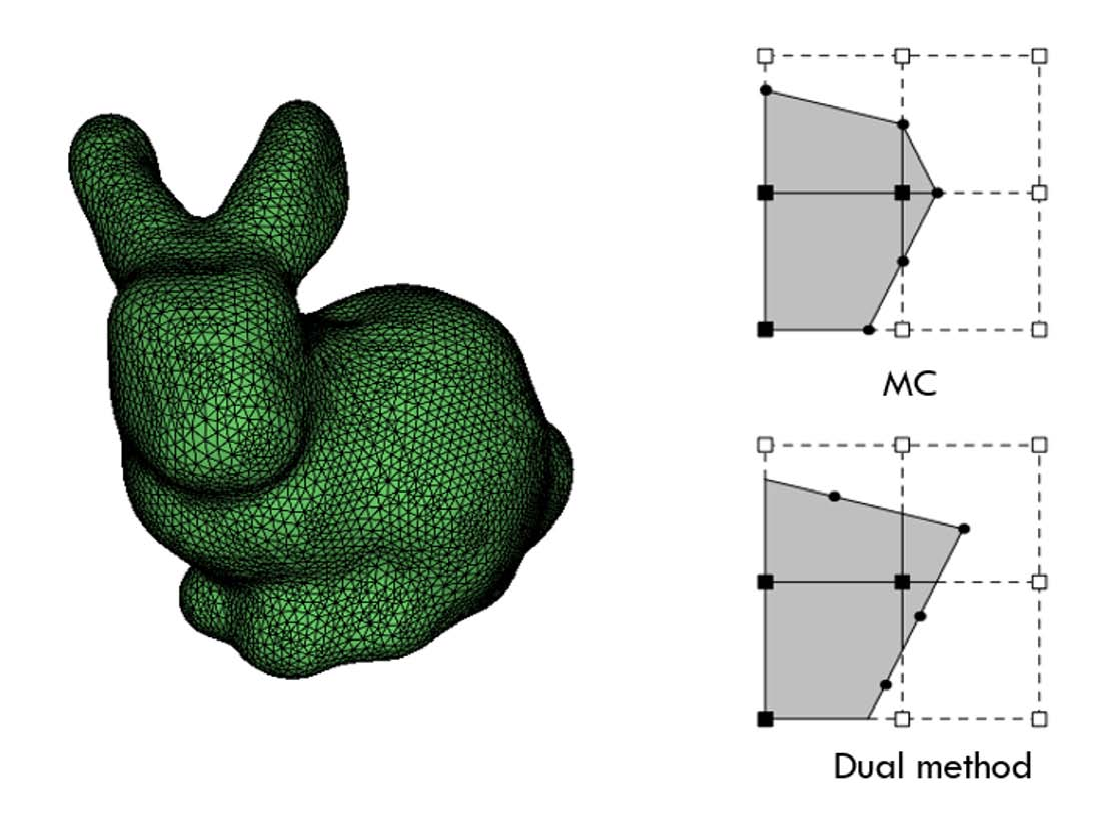
\includegraphics{Pictures/bunny_MC.pdf}}\\
   \caption{\textit{Left:} The famous Stanford Bunny, a popular computer graphics test object, here after application of Marching Cubes. \textit{Right:} Main difference between MC and Dual methods.  Figures taken from \cite{Hermite2002}. }
   \label{fig:bunny_MCDC}
\end{figure}
%The VTK toolbox was used in order to implement the algorithms on our optimized data. It is a heavily object
%oriented toolbox. Our first approach was to use the built in Marching Cubes algorithm,
%nevertheless it did not work with our unstructured grid data. It just works for ImageData and
%PolyData . For structured and unstructured grids the tool to render the isosurface is the \textit{Contour Filter} tool. Unfortunately the documentation does not present which algorithm the tool uses. It
%can be inferred that it is an extended Marching cubes algorithm.



%It finally allowed visualization but it created one problem. Holes are lost in
%the process.